\chapter{Эллиптический бильярд с косинусным законом преломления на софокусных квадриках.}\label{ch:ch3}

\section{Предварительные сведения.}\label{sec:ch3/sec1}

\subsection{Классический бильярд.}\label{sec:ch3/sec1/sub1}

Зафиксируем большую и малую полуоси эллипса $a$ и $b$, где $a > b > 0$ и во внутренности эллипса $\left(f(x, y) = \dfrac{x^2}{a^2}+\dfrac{y^2}{b^2} < 1 \right)$ рассмотрим движение материальной точки с координатами $\mathbf{x} = (x, y)$ и вектором скорости $\mathbf{v} = (v_x, v_y)$, при котором на границе эллипса $f(x, y) = 1$ векторы скорости до отражения и после него образуют равные по величине углы с вектором нормали $n=\left.\nabla f(x,y)\right|_{(x_0,y_0)} = \left( \dfrac{2x_0}{a^2},\dfrac{2y_0}{b^2}\right)$ к эллипсу в точке отражения $(x_0, y_0)$.

Обозначим $\Psi = \left\{ Q_{\lambda} \ |\ \lambda \in (0, a^2) \right\}$ -- однопараметрическое семейство софокусных квадрик, где квадрика $Q_\lambda$ задается уравнением 
$$f_\lambda(x,y)=\dfrac{x^2}{a^2-\lambda} + \dfrac{y^2}{b^2-\lambda} = 1.$$

Интегрируемость классического бильярда обусловлена классической теоремой из геометрии: если какое-то звено бильярдной траектории коснулось софокусной квадрики $Q_\lambda$ из семейства $\Psi$, то и все остальные звенья касаются этой же квадрики, поэтому $\lambda$ является первым интегралом.


\subsection{Интеграл Иоахимсталя.}\label{sec:ch3/sec1/sub2}
Пусть $M = Q_0 \times \mathbb{R}^2$ -- фазовый цилиндр бильярда в эллипсе $Q_0$. Для точки $(\mathbf{x}, \mathbf{v}) = ((x,y), (v_x, v_y)) \in M$ рассмотрим функцию $J(\mathbf{x}, \mathbf{v}) = -\left(
\frac{x v_x}{a^2} + \frac{y v_y}{b^2} \right).$
Функция $J(\mathbf{x}, \mathbf{v})$ не является интегралом движения точки в эллиптическом бильярде, так как не сохраняется на прямолинейных отрезках траектории. Тем не менее, для <<дискретного>> бильярда в эллипсе, когда траектория записывается последовательностью точек на эллипсе, в которых траектории испытывают отражения, функция $J(\mathbf{x}, \mathbf{v})$ является интегралом. А именно, прямолинейное звено бильярдной траектории будем кодировать начальной точкой звена $(x, y)$ и его вектором скорости $(v_x, v_y)$. Тогда выполняется следующее утверждение: 

\begin{theorem}{\normalfont{[7, с.~61]}}.
Пусть $(\mathbf{x}_i, \mathbf{v}_i) \in M, \quad i=1,\ldots$, -- последовательность точек на фазовом цилиндре, кодирующая последовательные звенья некоторой  бильярдной траектории. Тогда $J(\mathbf{x}_i, \mathbf{v}_i) =  J(\mathbf{x}_{i+1}, \mathbf{v}_{i+1})$ для всех $i$.
\label{th:sect3_th1}
\end{theorem}

Функцию $J$ называют интегралом Иоахимсталя. Заметим, что эту функцию можно переписать в виде 
$$J(\mathbf{x}, \mathbf{v}) = -\frac{1}{2}\langle\mathbf{v}, \nabla f_0(x, y)\rangle,$$
где $\langle\cdot, \cdot\rangle$ обозначает скалярное произведение. 

Прежде чем перейти к геометрическому смыслу интеграла Иоахимсталя, рассмотрим следующий вопрос: сколько квадрик из семейства $\Psi = \left\{ Q_{\lambda} \ |\ \lambda \in (0, a^2) \right\}$ касаются   фиксированной произвольным образом прямой в $\mathbb{R}^2$?

\begin{statement}
Рассмотрим прямую $\mathbf{x}+t\mathbf{v}$, проходящую через точку $\mathbf{x}= (x, y)$ на плоскости $\mathbb{R}^2$ и имеющую направление $\mathbf{v}=(v_x, v_y)$. Тогда:

$(i)$ Прямая касается не более одной квадрики $Q_\lambda$ из семейства $\Psi$.

$(ii)$ Исключая вертикальную ось $x=0$ и прямые, проходящие хотя бы через один из фокусов,  такая касательная квадрика  $Q_\lambda$ существует и ее параметр $\lambda$ определяется по формуле 
\begin{equation}
\lambda = \Lambda(\mathbf{x}, \mathbf{v}) = \frac{a^2 v_y^2 + b^2v_x^2 - (x v_y-y v_x)^2}{v_x^2 + v_y^2}.
\label{eq:sect3_eq1}
\end{equation}

\end{statement}

\begin{proof}
Прямая $\mathbf{x} + t \mathbf{v}$ касается квадрики $Q_\lambda$ тогда и только тогда, когда уравнение
$$\frac{(x + t v_x)^2}{a^2-\lambda} + \frac{(y + t v_y)^2}{b^2-\lambda} = 1$$
имеет ровно одно решение по $t$, то есть когда дискриминант квадратного уравнения с переменной $t$  равен нулю. Приравнивая дискриминант к нулю и решая равенство относительно параметра софокусной квадрики $\lambda$ можно получить формулу \eqref{eq:sect3_eq1} из второго пункта формулировки утверждения. В случаях, если $\lambda = a^2$ или $\lambda = b^2$, касательная квадрика $Q_\lambda$ вырождается в прямую (проходящую через малую полуось при $\lambda = a^2$ и проходящая через большую полуось при $\lambda = b^2$), следовательно прямая $\mathbf{x}+ t\mathbf{v}$ не касается никакой софокусной квадрики $Q_\lambda$.
\end{proof}

Заметим, что для бильярда в эллипсе вычисленный в точке $(\mathbf{x}, \mathbf{v})$ фазового цилиндра $M$ интеграл Иоахимсталя связан с параметром софокусной квадрики $\lambda$, которой касается прямая с направляющим вектором $\mathbf{v}$, проходящая через точку $\mathbf{x}$.

\begin{statement}
    Пусть $(\mathbf{x}, \mathbf{v})$ кодируют некоторое звено бильярдной траектории. Пусть $\lambda$ -- параметр квадрики $Q_\lambda$, касающейся прямой $\mathbf{x} +t \mathbf{v}$. Тогда 
    \begin{equation}
        \lambda = \Lambda(\mathbf{x}, \mathbf{v}) =  a^2 b^2 \frac{J^2(\mathbf{x}, \mathbf{v})}{||\mathbf{v}||^2}
    \label{eq:sect3_eq2}
    \end{equation}
\end{statement}

\begin{proof}
Выражение \eqref{eq:sect3_eq1} для $\lambda$ перепишем, домножив обе части на знаменатель:
\begin{equation}
(v_x^2 + v_y^2)\lambda = a^2 v_y^2 + b^2v_x^2 - (x v_y-y v_x)^2 = (a^2-x^2)v_y^2 + (b^2-y^2)v_x^2 + 2 x y v_x v_y.
\label{eq:sect3_eq3}
\end{equation}
Точка $(x, y)$ находится на эллипсе $Q_0$, поэтому
\begin{equation}
a^2 - x^2 = \frac{a^2 y^2}{b^2} \text{  и } b^2 - y^2 = \frac{b^2 x^2}{a^2}.
\label{eq:sect3_eq4}
\end{equation}
Подставляя \eqref{eq:sect3_eq4} в \eqref{eq:sect3_eq3}, получаем
$$||\mathbf{v}||^2 \lambda = \frac{a^2y^2}{b^2} + \frac{b^2 x^2}{a^2} + 2 x y v_x v_y = ||\mathbf{v}||^2 a^2b^2 \left( \frac{x v_x}{a^2} + \frac{y v_y}{b^2}\right)^2 = a^2b^2J^2(\mathbf{x}, \mathbf{v}).$$
\end{proof}

\section{Косинусный закон преломления.}\label{sec:ch3/sec2}
Пусть две области $\Omega_i$ и $\Omega_j$ граничат по кривой $C$. 
Показатели преломления для этих областей равны $n_i$ и $n_j$, соответственно.
Будем считать, что движение материальной точки при достижении кривой $C$ подчиняется следующим правилам (далее мы будем ссылаться на них как на модифицированный закон преломления $(\ast)$).
\begin{itemize}
\item[1.] Выполнено соотношение $n_i \cos \theta_i = n_j \cos \theta_j $, где $\theta_i, \theta_j \in [0,\frac{\pi}{2} ]$ -- углы, которые образуют отрезки траектории   в соответствующих областях с нормалью к кривой $C$, если $\theta_i$ и $\theta_j$ корректно определены.
\item[2.] Если $n_i > n_j$ и материальная точка, двигаясь в области $\Omega_i$, достигает кривой $C$, причем в точке пересечения траектории с кривой $C$ выполнено неравенство $\cos \theta_i > \frac{n_j}{n_i}$, то происходит полное внутреннее отражение траектории в область $\Omega_i$ по закону <<угол падения равен углу отражения>> (в этом случае угол $\theta_j$ не определен, поскольку $\frac{n_i}{n_j} \cos \theta_i > 1$). 
\item[3.] В предыдущих двух пунктах два соседних отрезка траектории с общей точкой на кривой $C$ лежат по разные стороны от нормали к кривой $C$ в этой точке.
\item[4.] Если $n_i > n_j$ и материальная точка, двигаясь в области $\Omega_j$, достигает кривой $C$, причем $\theta_j = 0$, тогда $\cos \theta_i = \frac{n_j}{n_i}$ и материальная точка продолжает движение в области $\Omega_i$ вдоль любого из двух возможных направлений, образующих угол $\theta_i$ с нормалью к кривой $C$.
\item[5.] Аналогично при $n_i < n_j$.
\end{itemize}
Для удобства будем считать, что при преломлении модуль вектора скорости не меняется.

\begin{figure}[!htb]
\minipage{0.32\textwidth}
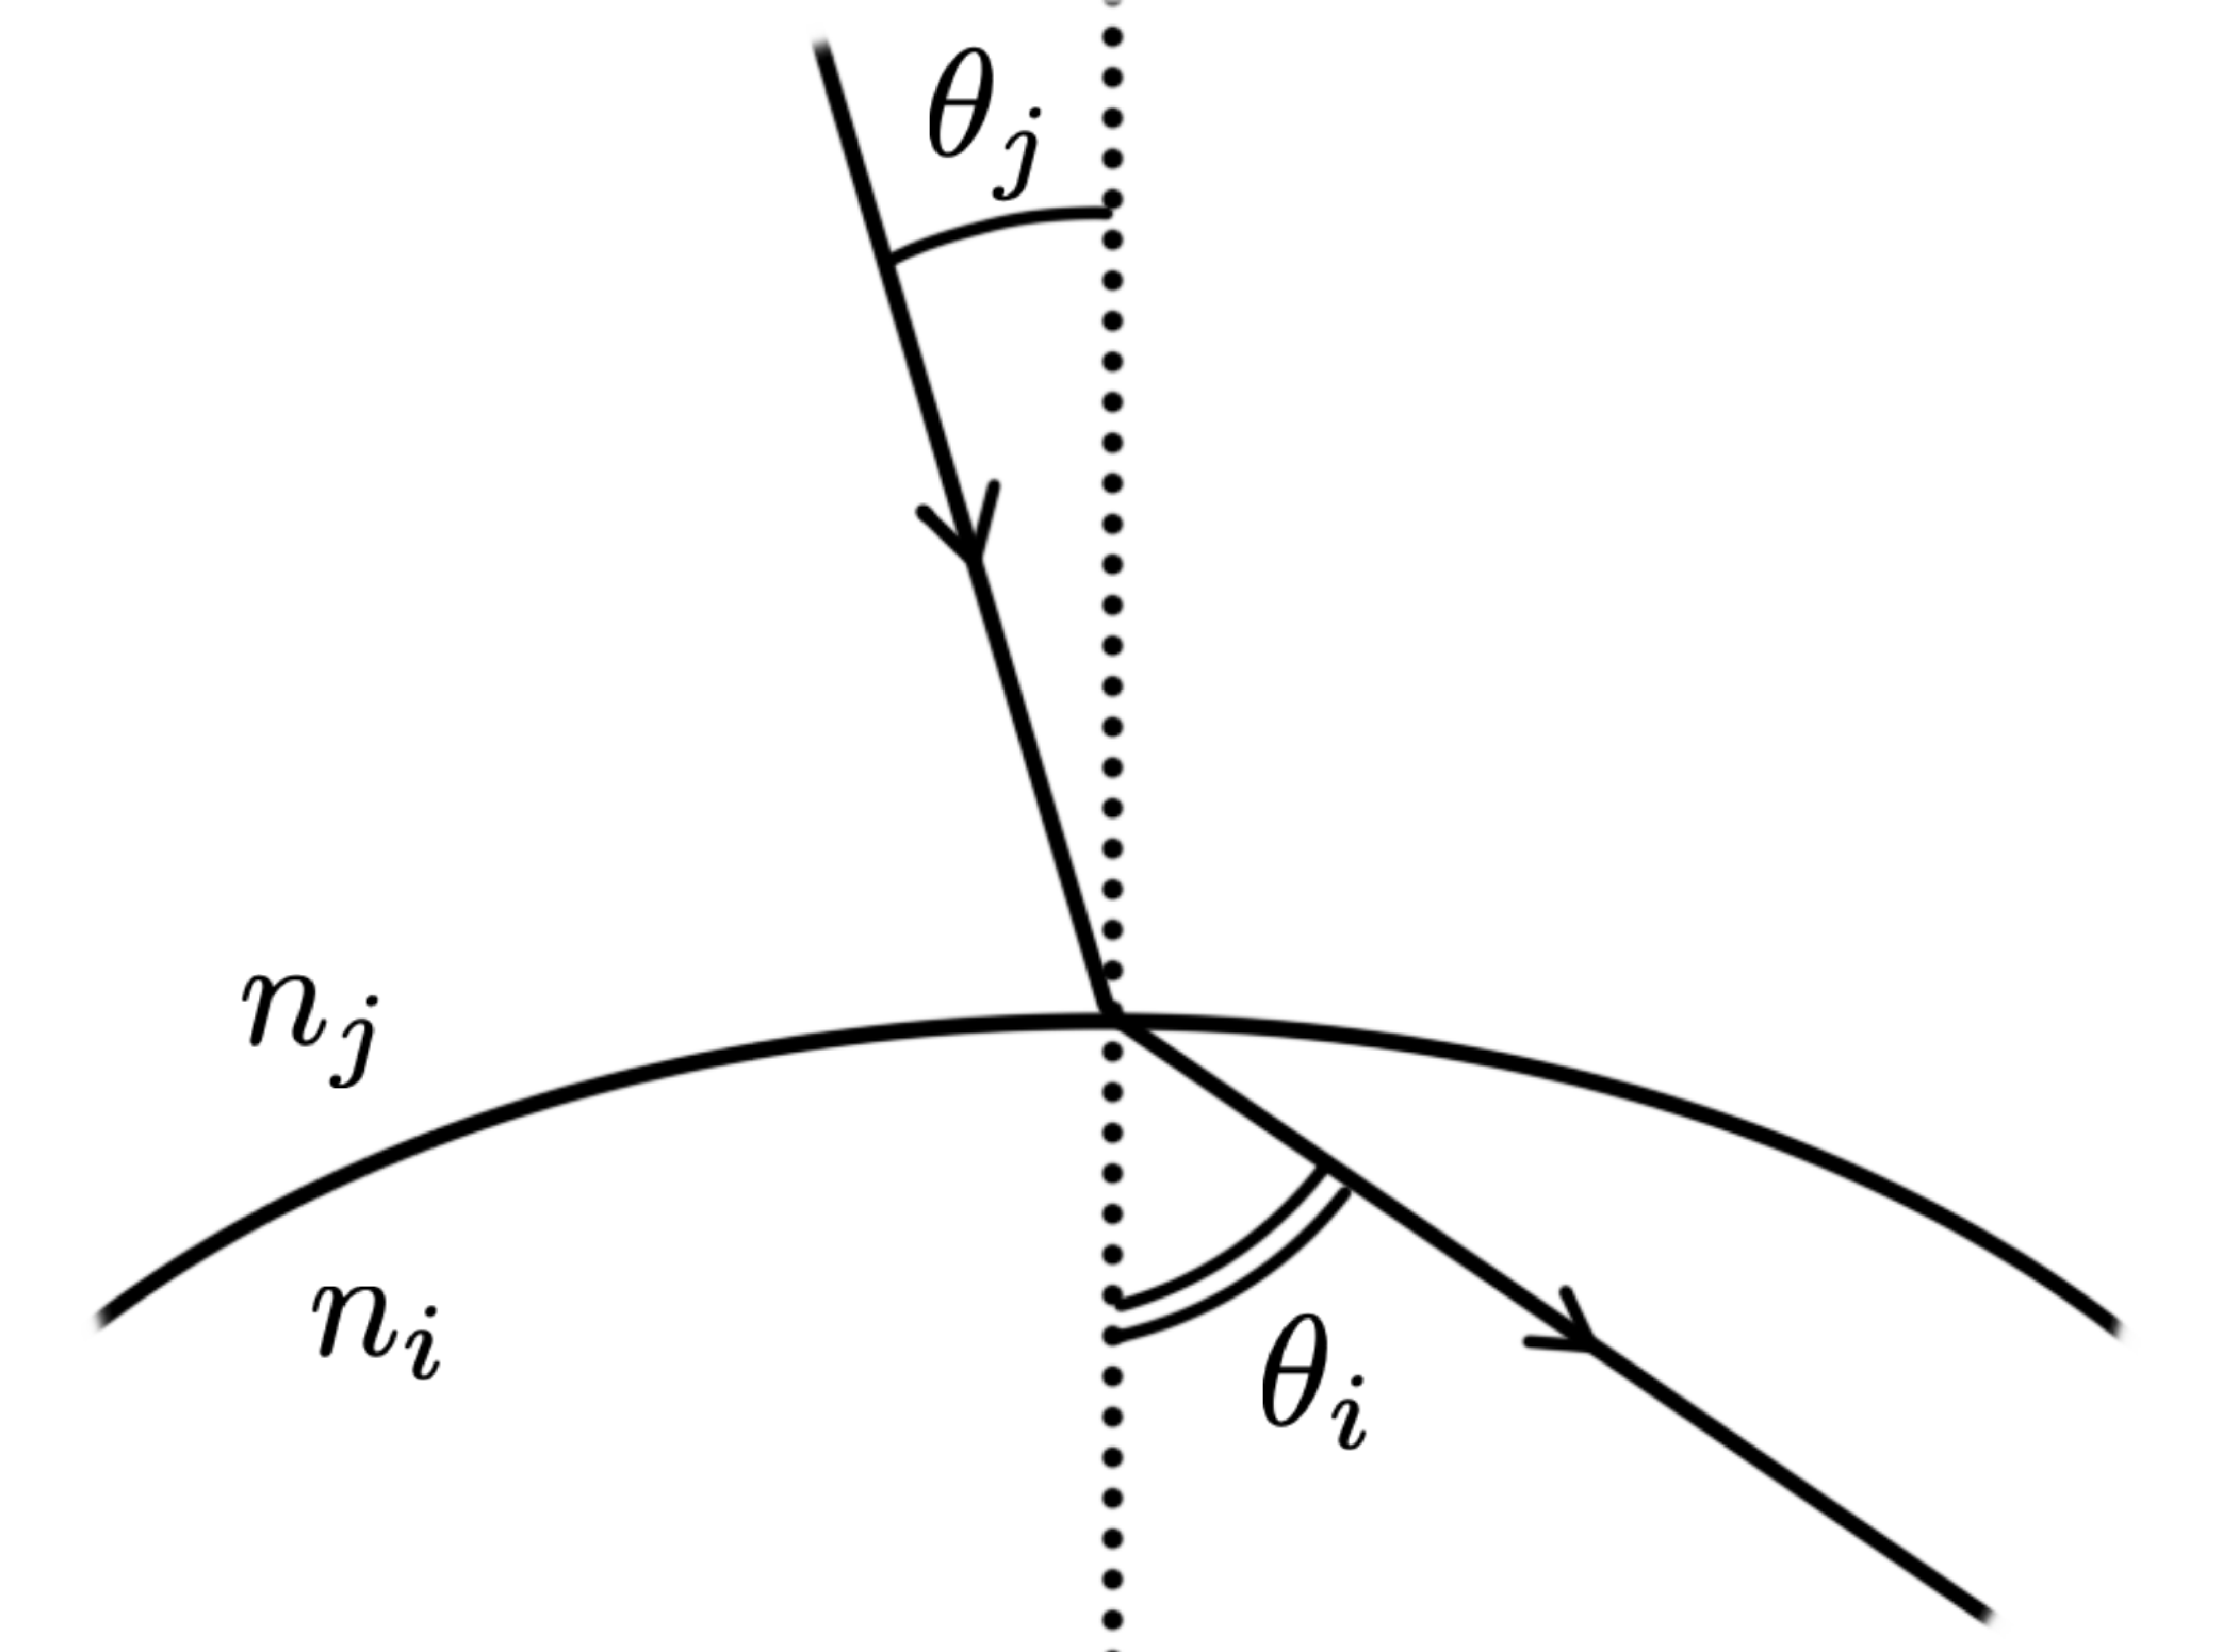
\includegraphics[width=\linewidth]{images/ch4/section1/example1.pdf}
    \caption{Иллюстрация к пункту 1.}
    \label{fig:pt8:_example1}
\endminipage\hfill
\minipage{0.32\textwidth}
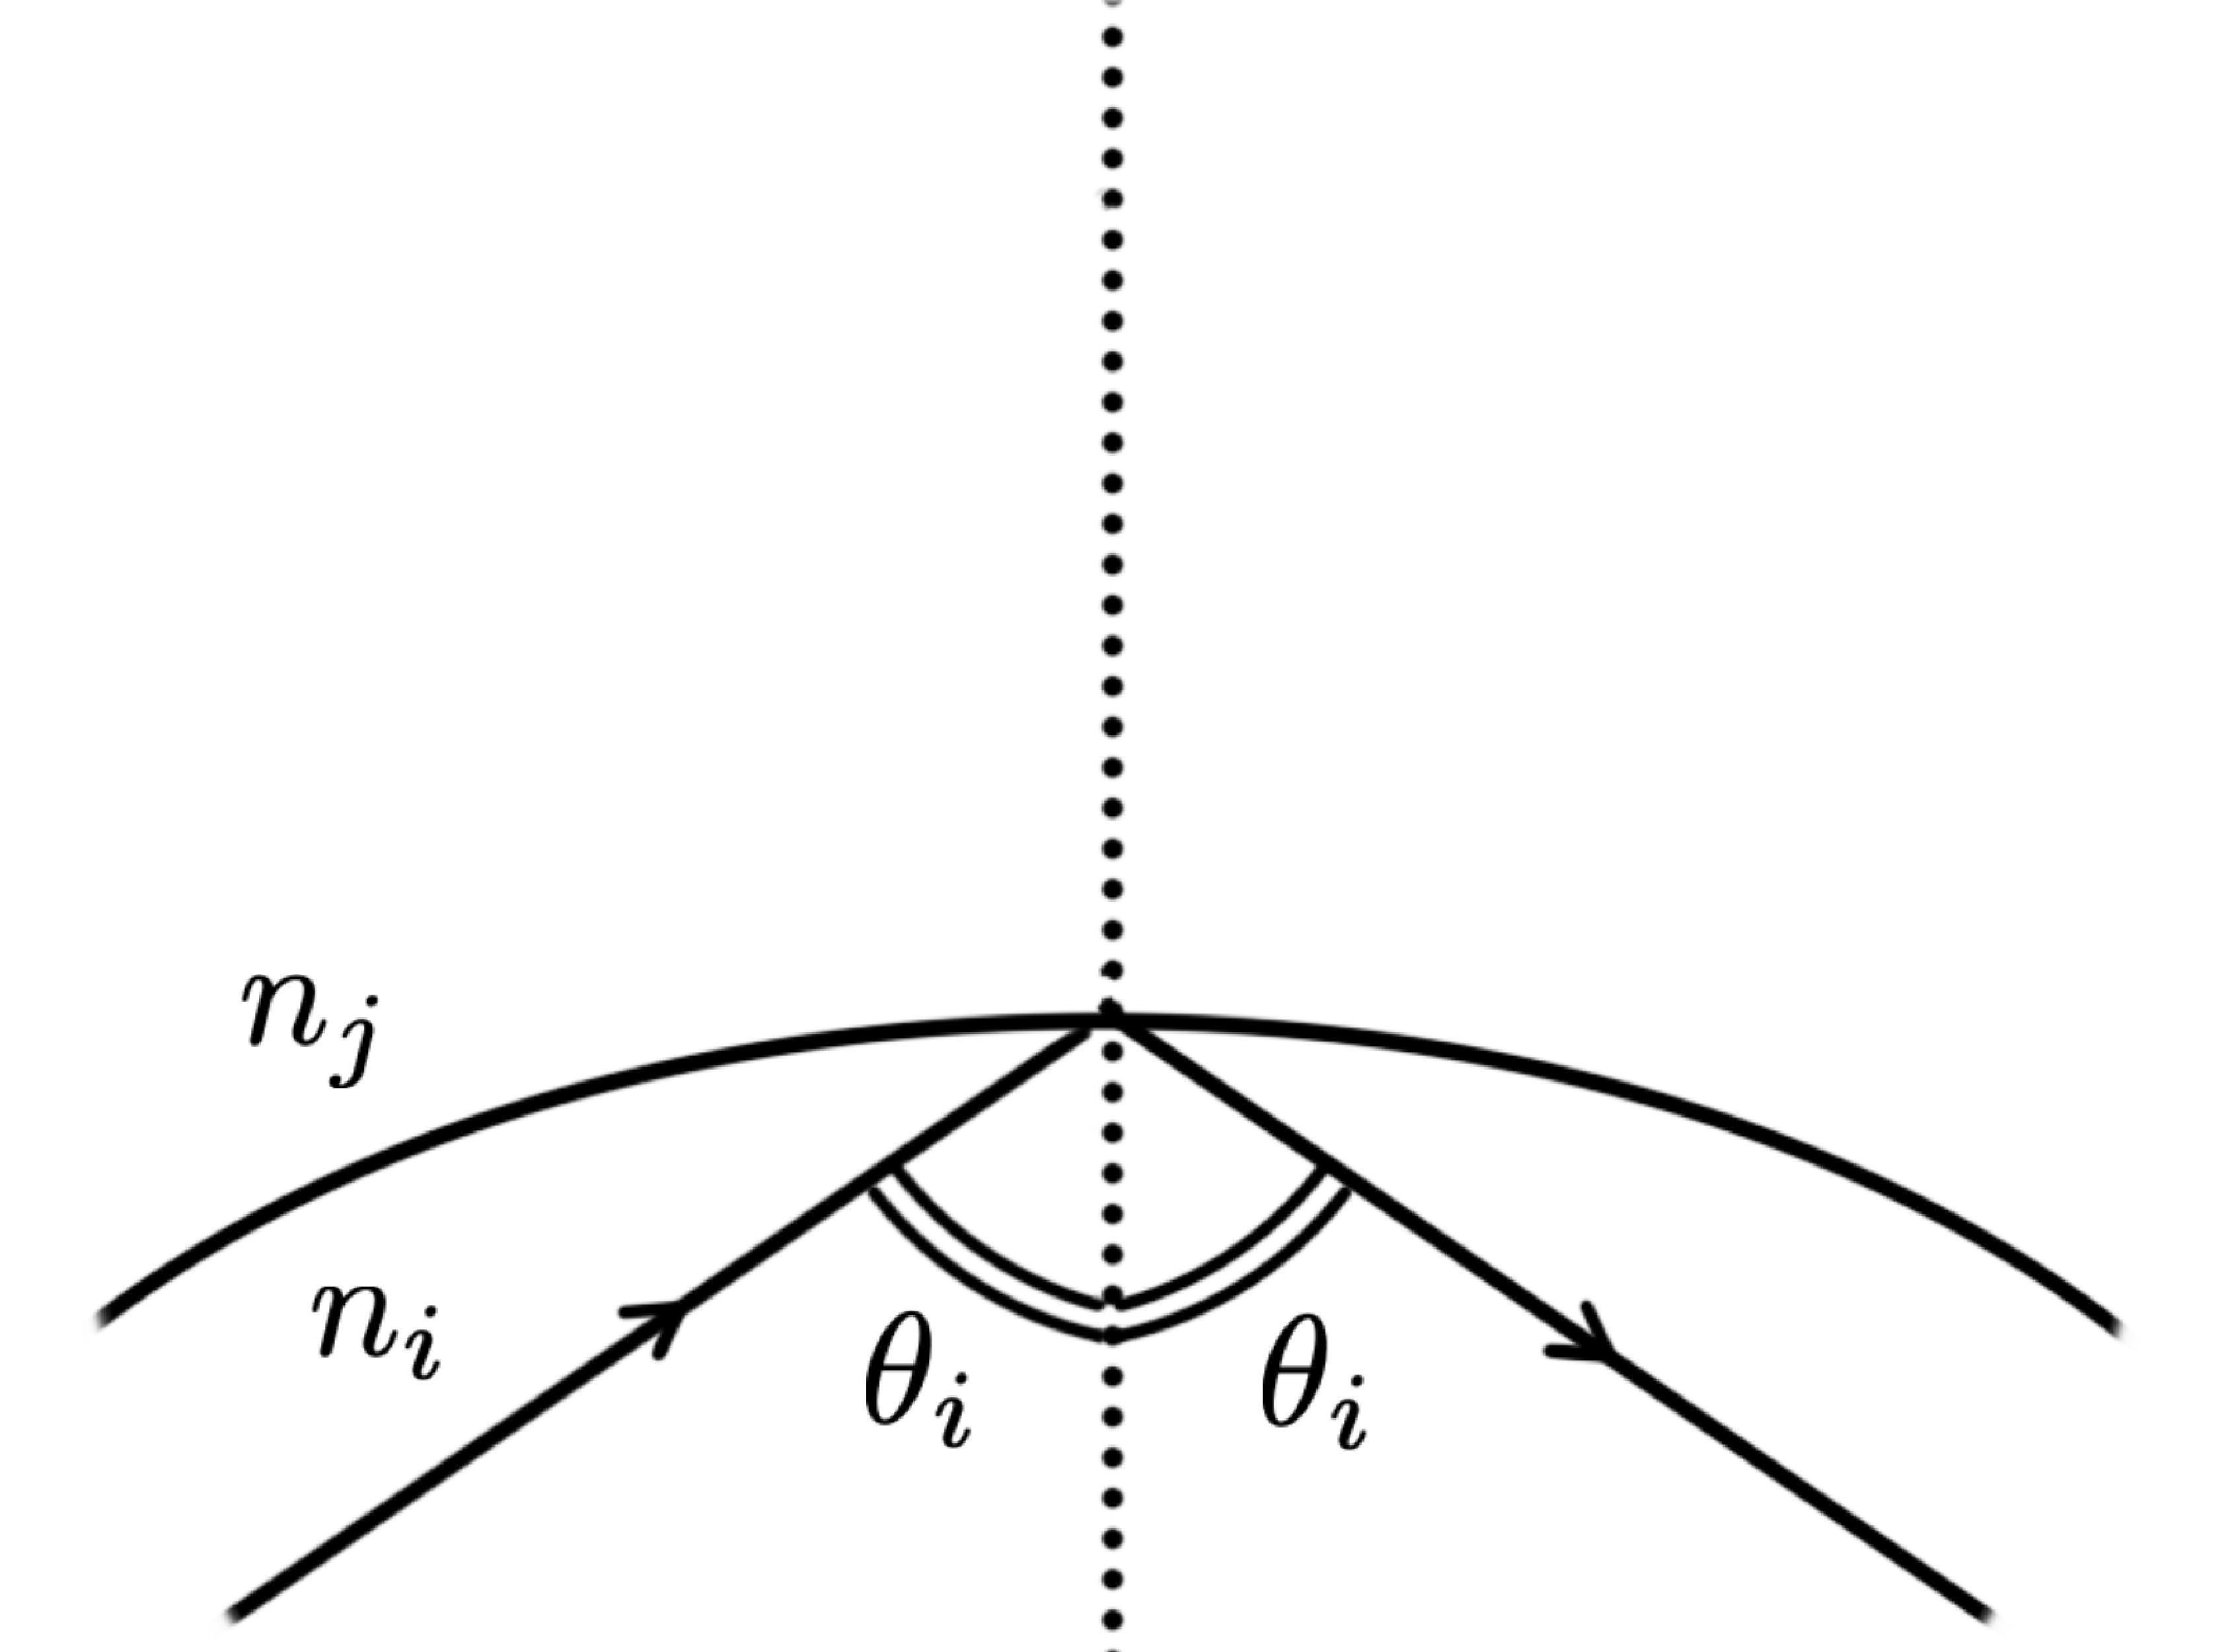
\includegraphics[width=\linewidth]{images/ch4/section1/example2.pdf}
    \caption{Иллюстрация к пункту 2.}
    \label{fig:pt8:_example2}
\endminipage\hfill
\minipage{0.32\textwidth}
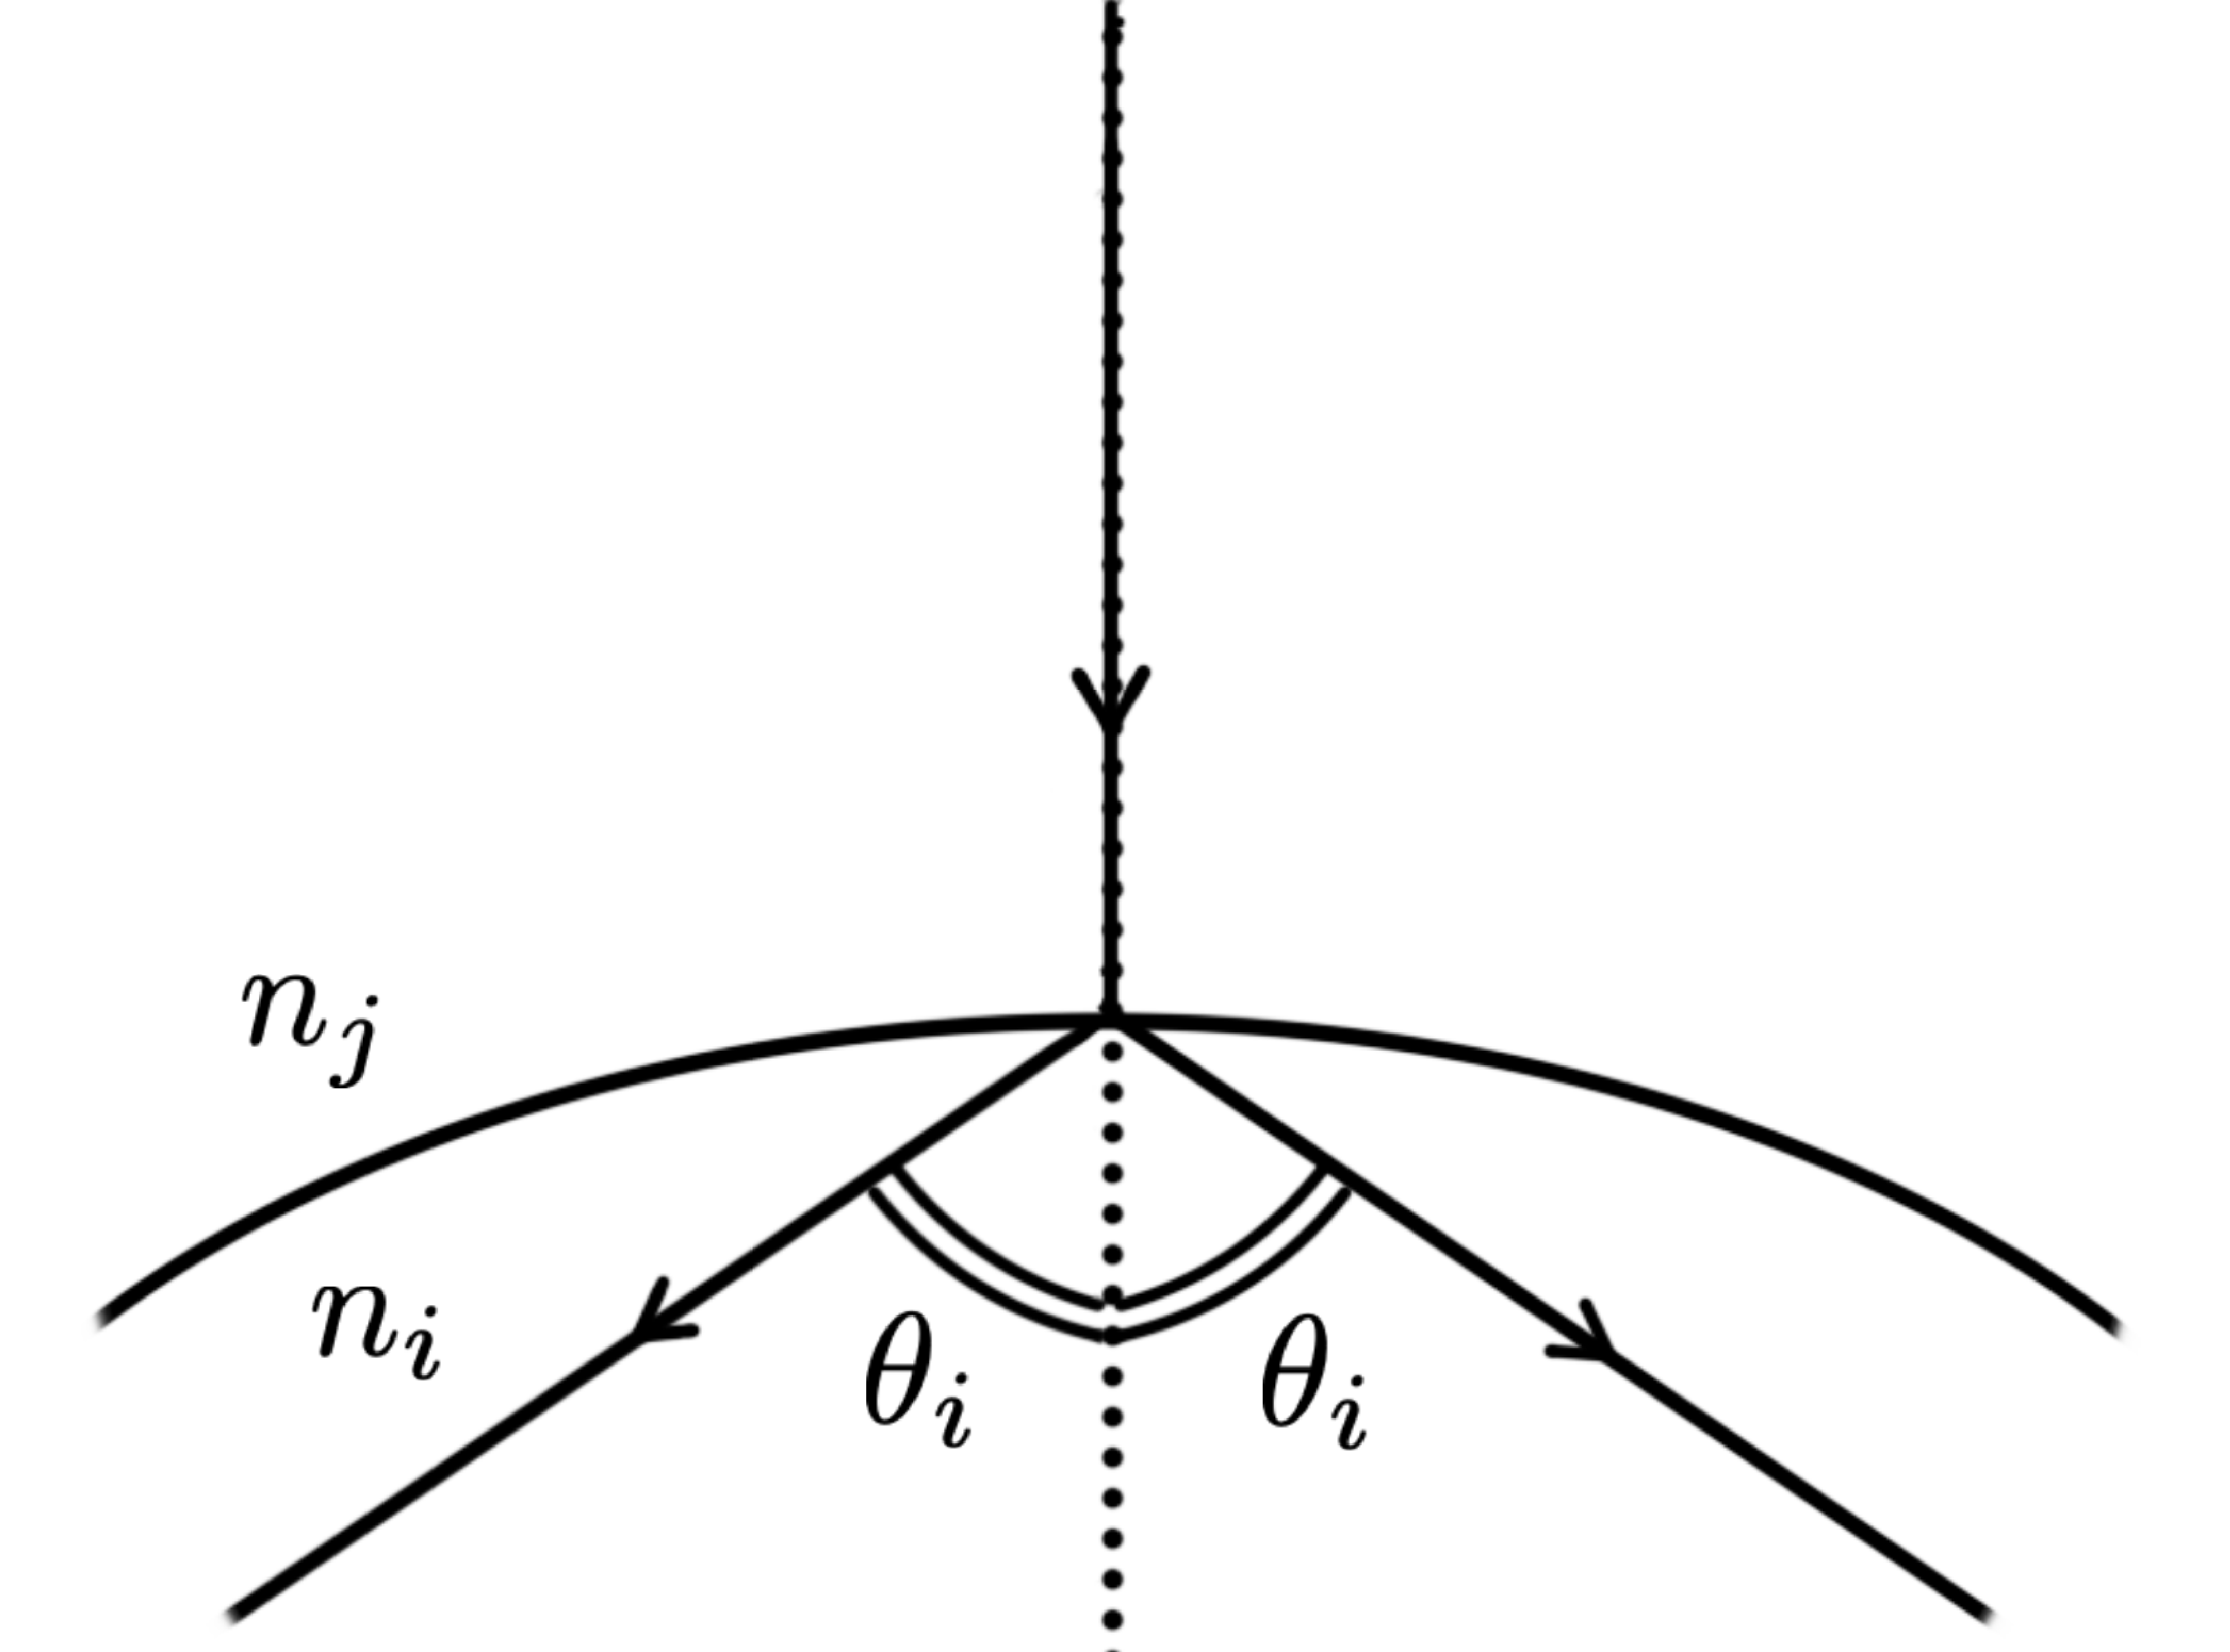
\includegraphics[width=\linewidth]{images/ch4/section1/example3.pdf}
    \caption{Иллюстрация к пункту 4.}
    \label{fig:pt8:_example3}
\endminipage\hfill
\end{figure}

\subsection{Постоянная движения}\label{sec:ch3/sec3}
Пусть задана область $\Omega$, ограниченная эллипсом 
$\dfrac{x^2}{a^2} + \dfrac{y^2}{b^2} = 1$, где $a > b > 0$.
Дуга софокусной квадрики $Q_{\lambda_0} = \left\{ \dfrac{x^2}{a^2-\lambda_0} + \dfrac{y^2}{b^2-\lambda_0} = 1 \right\}$ разделяет  $\Omega$ на области $\Omega_1$ и $\Omega_2$.
В случае $0 < \lambda_0 < b^2$ квадрика $Q_{\lambda_0}$ является эллипсом, а при $b^2 < \lambda_0 < a^2$ -- гиперболой.

Припишем каждой области $\Omega_i$  коэффициент $n_i,\  i=1,2$, имеющий смысл показателя преломления. 
Рассмотрим движение материальной точки в области $\Omega$. Будем считать, что на внешней границе области $\Omega$ движение подчиняется закону <<угол падения равен углу отражения>>, 
а на общей границе областей $\Omega_1$ и $\Omega_2$ выполняется модифицированный закон преломления $(\ast)$.

Определим функцию $\Xi(x, y, v_x, v_y)$ положения и скорости материальной точки (в декартовых координатах) по формуле
\begin{equation}
\Xi(x, y, v_x, v_y) = \left[
\begin{array}{ll}
    \Lambda(x, y, v_x, v_y) n_1^2, &  \text{ если } (x,y) \in \Omega_1 \\
    \Lambda(x, y, v_x, v_y) n_2^2 + \lambda_0 (n_1^2-n_2^2), & \text{ если } (x,y) \in \Omega_2    .
\end{array}
\right.
\label{eq:xi_integral_definition}
\end{equation}
Здесь величина $\Lambda(x, y, v_x, v_y)$ определена как в уравнении \eqref{eq:sect3_eq1} и имеет смысл коэффициента $\alpha$  софокусной квадрики $Q_\alpha$, которая касается прямой, проходящей через точку $(x,y)$ в направлении вектора $(v_x, v_y)$.

Функция $\Xi(x, y, v_x, v_y)$ является первым интегралом рассматриваемой динамической системы в области $\Omega$.
Доказательство изложено в разделе \ref{sec:ch3/sec3/sub2}.

\subsubsection{Вспомогательные утверждения}\label{sec:ch3/sec3/sub1}

 \begin{statement}
Пусть $\mathbf{n}$ -- вектор нормали разделяющей среды кривой $C$ в точке преломления $(x_0, y_0)$, а также пусть $\mathbf{v}$ -- вектор скорости до преломления. Считаем, что траектория бильярда в точке $(x_0, y_0)$ переходит из среды с показателем преломления $n_1$ в область с показателем $n_2$. Тогда если вектор $\mathbf{v}$ не параллелен вектору $\mathbf{n}$, то для вектора   $\mathbf{w}$  после преломления справедливо выражение 
$\mathbf{w} = \alpha \mathbf{v} + \beta \mathbf{n}$, где 
$$\beta = \dfrac{||\mathbf{w}|| \mu - ||\mathbf{v}|| \alpha}{||\mathbf{n}||}\cos{\theta_1}, \ \alpha = \dfrac{||\mathbf{w}||}{||\mathbf{v}||}\sqrt{\dfrac{1-\mu^2\cos^2 \theta_1}{1-\cos^2 \theta_1 }},$$  $\theta_1$ -- угол, образованный векторами $\mathbf{v}$ и $\mathbf{n}$, $\mu = \dfrac{n_1}{n_2}$.
\label{st:alpha_beta_cosine_law}
\end{statement}
\begin{proof}
Из закона преломления $(\ast)$ следует 
$\langle\mathbf{w}, \mathbf{n}\rangle = ||\mathbf{w}||\, ||\mathbf{n}|| \cos \theta_2 = ||\mathbf{w}||\, ||\mathbf{n}|| \mu \cos \theta_1$.

В то же время, из линейности скалярного произведения
$\langle\mathbf{w}, \mathbf{n}\rangle = \alpha \langle\mathbf{v}, \mathbf{n}\rangle + \beta\, ||\mathbf{n}||^2 = \alpha ||\mathbf{v}||\, ||\mathbf{n}|| \cos \theta_1 + \beta\, ||\mathbf{n}||^2$, следовательно, $\beta = \dfrac{||\mathbf{w}|| \mu - ||\mathbf{v}|| \alpha}{||\mathbf{n}||}\cos{\theta_1}$. 

Подставляя полученное значение $\beta$ в равенство $||\mathbf{w}||^2 = ||\alpha \mathbf{v} + \beta \mathbf{n}||^2 = \alpha^2 ||\mathbf{v}||^2 (1-\cos^2 \theta_1) + \mu^2||\mathbf{w}||^2 \cos^2 \theta_1$, получим нужную формулу для  $\alpha$.
\end{proof}

\begin{remark}
    Эти формулы очевидным образом упрощаются для $||\mathbf{n}|| = 1$ и $||\mathbf{v}|| = ||\mathbf{w}||$. В дальнейшем мы будем использовать эти формулы при $||\mathbf{v}|| = ||\mathbf{w}||$, но $||\mathbf{n}|| \neq 1$.
\end{remark}

\begin{statement}
Если траектория подходит к границе раздела сред $Q_{\lambda_0}$ под прямым углом (т.е. вектор скорости $\mathbf{v}$ пропорционален вектору нормали $\mathbf{n}$   квадрики $Q_{\lambda_0}$ в точке преломления $(x_0,y_0)$) и коэффициенты преломления не дают полное отражение (то есть $n_1 \cos \theta_1 = n_1 \leq n_2$), то вектор скорости после преломления может быть определен предельным переходом:
\begin{multline*}
\dfrac{\mathbf{w}}{||\mathbf{w}||} - \mu \dfrac{\mathbf{n}}{||\mathbf{n}||}=  \sqrt{\dfrac{1-\mu^2 \cos^2 \theta_1 }{1-\cos^2\theta_1}} \left( \dfrac{\mathbf{v}}{||\mathbf{v}||} - \dfrac{\mathbf{n}}{||\mathbf{n}||} \right) = \\
=  \sqrt{\dfrac{1-\mu^2 \cos^2 \theta_1 }{\sin^2\theta_1}}  \left(
    \begin{array}{cc}
    \cos \theta_1 - 1 \ & -\sin \theta_1 \\
    \sin \theta_1 \ & \cos \theta_1 - 1 
    \end{array}
\right) \dfrac{\mathbf{n}}{||\mathbf{n}||} = \\
=  \sqrt{1-\mu^2 \cos^2 \theta_1 }  \left(
    \begin{array}{cc}
    -\tan \frac{\theta_1}{2}  \ & -1 \\
    1 \ & -\tan \frac{\theta_1}{2}
    \end{array}
\right) \dfrac{\mathbf{n}}{||\mathbf{n}||} \ \xrightarrow[\theta_1 \to 0+]{} \ 
\sqrt{1-\mu^2}  \left(
    \begin{array}{cc}
    0  \ & -1 \\
    1  \ & 0
    \end{array}
\right) \dfrac{\mathbf{n}}{||\mathbf{n}||},
\end{multline*}
что эквивалентно пункту 4 закона $(\ast)$.
\end{statement}


\begin{statement}
Рассмотрим точку $\mathbf{x}=(x, y) \in Q_{\lambda_0}$ и пару векторов скоростей $\mathbf{v}$, $\mathbf{w}$ до и после преломления в точке $\mathbf{x}$, соответственно. 
Имеет место равенство
\begin{equation}
\dfrac{n_2 J_{\lambda_0}(\mathbf{x}, \mathbf{w})}{||\mathbf{w}||} = 
\dfrac{n_1 J_{\lambda_0}(\mathbf{x}, \mathbf{v})}{||\mathbf{v}||}.
\label{eq:sect3_eq7}
\end{equation}
%$\frac{J_{\lambda_0}(\mathbf{x}, \mathbf{w})}{||\mathbf{w}||} = \mu \frac{J_{\lambda_0}(\mathbf{x}, \mathbf{v})}{||\mathbf{v}||}$
\label{th:joachFraction}
\end{statement}

%\begin{remark}
%Мы записали основное равенство в этом утверждении именно в такой форме, чтобы  была очевидна связь с формулой \eqref{eq:sect3_eq2} для $\Lambda(\mathbf{x}, \mathbf{v})$.
%\end{remark}
\begin{proof}
Из определения функции $J_{\lambda_0}$ следует равенство $J_{\lambda_0}(\mathbf{x}, \mathbf{v}) = -\frac{1}{2}||\mathbf{v}|| ||\mathbf{n}|| \cos \theta_1$, а с учетом формул для коэффициентов $\alpha$ и $\beta$ из утверждения \ref{st:alpha_beta_cosine_law} получаем 
\begin{multline*}
    J_{\lambda_0}(\mathbf{x}, \mathbf{w}) = \alpha J_{\lambda_0}(\mathbf{x}, \mathbf{v}) + \beta J_{\lambda_0}(\mathbf{x}, \mathbf{n}) = \alpha J_{\lambda_0}(\mathbf{x}, \mathbf{v}) - \frac{\beta}{2}||\mathbf{n}||^2 = \\ =\alpha J_{\lambda_0}(\mathbf{x}, \mathbf{v}) + ||\mathbf{n}||^2\frac{||\mathbf{w}||\mu-||\mathbf{v}||\alpha}{||\mathbf{n}||}\frac{J_{\lambda_0}(\mathbf{x}, \mathbf{v})}{||\mathbf{v}|| ||\mathbf{n}||} = 
\frac{||\mathbf{w}||}{||\mathbf{v}||}\mu J_{\lambda_0}(\mathbf{x}, \mathbf{v}),
\end{multline*}
где $\mu=\frac{n_1}{n_2}$. Следовательно, 
$
\frac{n_2 J_{\lambda_0}(\mathbf{x}, \mathbf{w})}{||\mathbf{w}||} = 
\frac{n_1 J_{\lambda_0}(\mathbf{x}, \mathbf{v})}{||\mathbf{v}||}.
$
\end{proof}

\begin{statement}
    
    $(i)$ При $\theta_1=0$ и $n_1 \leq n_2$ равенство
    \eqref{eq:sect3_eq7} тоже выполняется 
    
    $(ii)$ Более того, величины $J_{\lambda_0}(\mathbf{x}, \mathbf{w})$ для <<левой>> и <<правой>> траекторий совпадают.
\end{statement}
\begin{proof}

$(i)$ Поскольку $\mathbf{v} \| \mathbf{n}$, $||\mathbf{w}|| = ||\mathbf{v}||$,  то очевидно равенство 
    $$J_{\lambda_0}(\mathbf{x}, \mathbf{w}) 
    = -\frac{1}{2}||\mathbf{n}||||\mathbf{w}|| \cos \theta_2 
    = -\frac{1}{2}||\mathbf{n}||||\mathbf{v}|| \cos \arccos \frac{n_1}{n_2} 
    = \frac{n_1}{n_2} J_{\lambda_0}(\mathbf{x}, \mathbf{v}).$$

$(ii)$ В силу четности косинуса из определения $J_{\lambda_0}(\mathbf{x}, \mathbf{w})$ следует, что
\begin{multline*}
J_{\lambda_0}(\mathbf{x}, R(\theta_2) \mathbf{v})
=-\frac{1}{2}\langle\mathbf{n},  R(\theta_2) \mathbf{v}\rangle
=-\frac{1}{2}||\mathbf{n}||||\mathbf{v}|| \cos \theta_2 = \\
=-\frac{1}{2}||\mathbf{n}||||\mathbf{v}|| \cos -\theta_2 
=-\frac{1}{2}\langle\mathbf{n},  R(-\theta_2) \mathbf{v}\rangle
=J_{\lambda_0}(\mathbf{x}, R(-\theta_2) \mathbf{v}).
\end{multline*}
\end{proof}

\subsubsection{Постоянная движения $\Xi$ (доказательство)}\label{sec:ch3/sec3/sub2}
Вернемся к системе, описанной в разделе \ref{sec:ch3/sec3}.
\begin{theorem}
    Функция $\Xi(\mathbf{x}, \mathbf{v})$, определенная как в уравнении \eqref{eq:xi_integral_definition}, является постоянной на траекториях для бильярда с законом преломления $(\ast)$.
\label{th:xi_is_integral}
\end{theorem} 
\begin{proof}


Очевидно, что функция $\Xi(\mathbf{x}, \mathbf{v})$ является константой на каждом отрезке бильярдной траектории с преломлением, полностью лежащем в $\Omega_1$ или $\Omega_2$. Легко сообразить, что в момент отражения функция $\Xi(\mathbf{x}, \mathbf{v})$ также не меняет своего значения. Остается рассмотреть  момент преломления. С геометрической точки зрения удобно воспользоваться функцией  
$$J_{\lambda_0}(\mathbf{x}, \mathbf{v}) = -\left(\frac{x v_x}{a^2-\lambda_0} + \frac{y v_y}{b^2-\lambda_0} \right) = -\frac{1}{2}\langle\mathbf{v}, \nabla f_{\lambda_0}(x,y)\rangle,$$
определенной на дуге $\partial \Omega_1 \cap \partial \Omega_2$ квадрики $Q_{\lambda_0}$, заданной уравнением $f_{\lambda_0}(x, y) = 1$.

На дуге  $\partial \Omega_1 \cap \partial \Omega_2$ имеет место равенство
 $$\Lambda(\mathbf{x}, \mathbf{v})=(a^2-\lambda_0)(b^2-\lambda_0)\frac{J_{\lambda_0}(\mathbf{x}, \mathbf{v})^2}{||\mathbf{v}||^2}.$$

Рассмотрим траекторию бильярда в момент преломления. Для определенности предположим, что  до преломления частица движется в среде с коэффициентом преломления $n_1$ с вектором скорости $\mathbf{v}$, который меняется на вектор $\mathbf{w}$ после перехода в среду с коэффициентом преломления $n_2$. При движении в обратном порядке эти два звена меняются местами, а нижеследующие утверждения по-прежнему справедливы.

Сначала рассмотрим каустику для области, коэффициент преломления которой равен $n_1$: пусть $(x,y) \in Q_{\lambda_0}$ и прямая $\mathbf{x}+t \mathbf{v}$ касается квадрики с параметром $\alpha_1$. 


Перепишем выражение для $\Lambda$ (см. \eqref{eq:sect3_eq1}) эквивалентным способом:
\begin{equation}
\alpha_1 = \Lambda(\mathbf{x}, \mathbf{v}) = \frac{(a^2-x^2) v_y^2 + (b^2-y^2)v_x^2 +2 x y v_x v_y}{v_x^2 + v_y^2}.
\label{eq:sect3_eq8}
\end{equation}
Из условия $(x,y) \in Q_{\lambda_0}$, т.е. из равенства $\frac{x^2}{a^2-\lambda_0} + \frac{y^2}{b^2-\lambda_0} =1$, используя соотношения \eqref{eq:sect3_eq4}, получаем:
$$a^2-x^2=\frac{a^2-\lambda_0}{b^2-\lambda_0}y^2+\lambda_0 \ \text{ и }\  b^2-y^2 = \frac{b^2-\lambda_0}{a^2-\lambda_0}x^2+\lambda_0.$$
Подставим эти выражения в формулу \eqref{eq:sect3_eq8} для $\alpha_1$:
\begin{multline*}
\alpha_1 = \frac{\frac{a^2-\lambda_0}{b^2-\lambda_0}y^2v_y^2 + \lambda_0 v_y^2 + \frac{b^2-\lambda_0}{a^2-\lambda_0}x^2v_x^2 + \lambda_0 v_x^2 + 2x y v_x v_y}{v_x^2+v_y^2} = \\
=\lambda_0 + (a^2-\lambda_0)(b^2-\lambda_0)\dfrac{(\frac{x v_x}{a^2-\lambda_0} + \frac{y v_y}{b^2-\lambda_0})^2}{v_x^2 + v_y^2} = 
\lambda_0 + (a^2-\lambda_0)(b^2-\lambda_0)\frac{J_{\lambda_0}(\mathbf{x}, \mathbf{v})^2}{||\mathbf{v}||^2}.
\end{multline*}

Повторяя те же рассуждения для преломленного луча $\mathbf{w}$, для параметра каустики $\alpha_2 = \Lambda(\mathbf{x}, \mathbf{w})$ имеем 
\begin{equation}
\alpha_2 = \lambda_0 + (a^2-\lambda_0)(b^2-\lambda_0)\frac{J_{\lambda_0}(\mathbf{x}, \mathbf{w})^2}{||\mathbf{w}||^2} = \lambda_0 + (a^2-\lambda_0)(b^2-\lambda_0)\frac{J_{\lambda_0}(\mathbf{x}, \mathbf{v})^2}{||\mathbf{v}||^2} \left(\frac{n_1}{n_2}\right)^2.
\label{eq:sect3_eq9}
\end{equation}

В результате из равенств \eqref{eq:sect3_eq8} и \eqref{eq:sect3_eq9} следует, что $\Lambda(\mathbf{x}, \mathbf{v}) - \lambda_0 = (\Lambda(\mathbf{x}, \mathbf{w}) - \lambda_0)\left(\frac{n_2}{n_1}\right)^2$. 
\end{proof}


\section{Общий случай}\label{sec:ch3/sec3}
Утверждение теоремы \ref{th:xi_is_integral} для $\Xi(\mathbf{x}, \mathbf{v})$ оказывается верным в значительно более общей ситуации.
Пусть внутренность эллипса разбита попарно непересекающимися дугами софокусных квадрик на области $\Omega_1, \ldots, \Omega_k$.  Перенумеруем области так, чтобы общие границы имели только области с соседними номерами. Пусть $\lambda_j$ --- параметр софокусной квадрики, разделяющей $\Omega_j$ и $\Omega_{j+1}$, $j=1, \ldots, k-1$. Два возможных варианта показаны на рис. \ref{fig:pt8:_example4} и \ref{fig:pt8:_example5}. Здесь и далее показатель преломления для области $\Omega_j$ обозначается через $n_j$.
\begin{figure}[!htb]
\minipage{0.45\textwidth}
   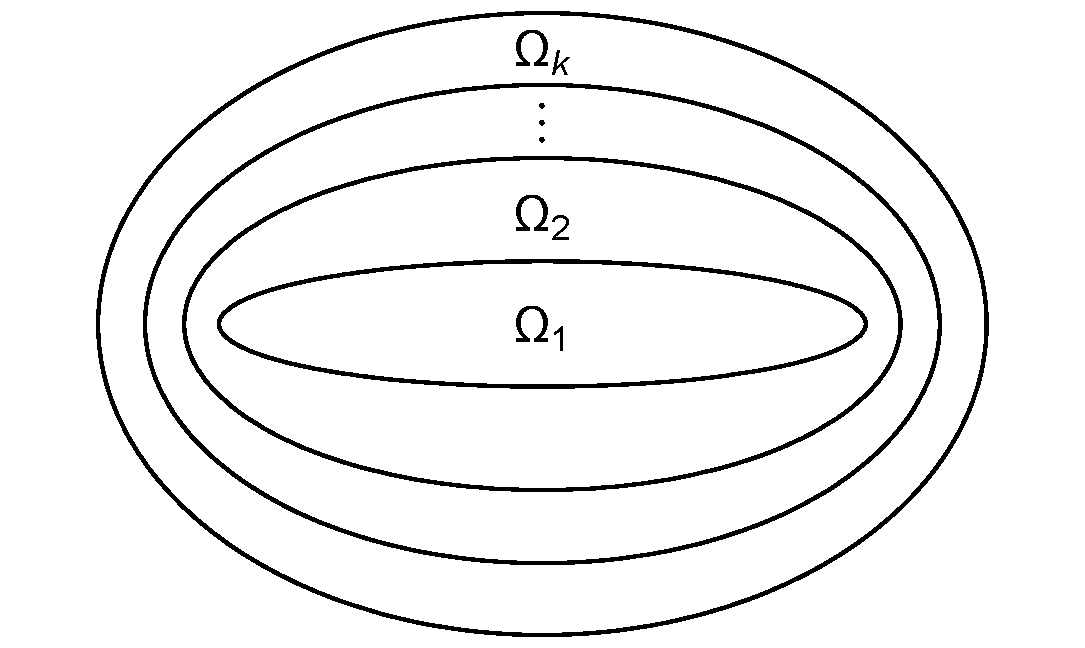
\includegraphics[width=1\textwidth]{images/ch4/section1/multiple ellipses.pdf}
    \caption{Взаимное расположение областей $\Omega_1, \ldots, \Omega_k$.}
    \label{fig:pt8:_example4}
\endminipage\hfill
\minipage{0.45\textwidth}
    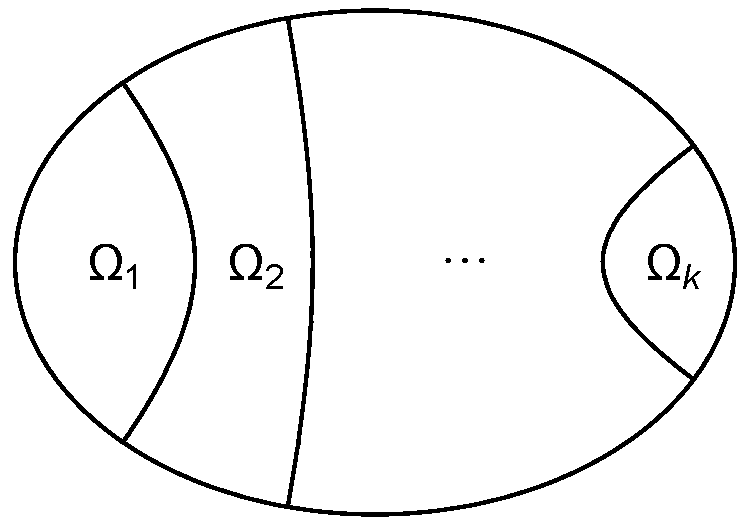
\includegraphics[width=0.9\textwidth]{images/ch4/section1/multiple hyperbolas.pdf}   
    \caption{Взаимное расположение областей $\Omega_1, \ldots, \Omega_k$.}
    \label{fig:pt8:_example5}
\endminipage\hfill
\end{figure}


Определим функцию $\Xi(x, y, v_x, v_y)$ по формуле: 
\begin{equation*}
\Xi(x, y, v_x, v_y) = \left[
\begin{array}{ll}
    \Lambda(x, y, v_x, v_y) n_1^2, \qquad  \ \ \qquad   \text{ если } (x,y) \in \Omega_1 ;
    \\
    \Lambda(x, y, v_x, v_y) n_p^2 + \sum_{j=1}^{p-1} \lambda_j(n_j^2-n_{j+1}^2), \\
     \qquad \qquad \qquad \qquad \qquad \qquad  \text{ если } (x,y) \in \Omega_p \text{ для } 1 < p \leq k. 
\end{array}
\right.
\end{equation*}

\begin{theorem}[\cite{vestnikLatest}]
Функция $\Xi(x, y, v_x, v_y)$ является константой на траекториях бильярда с модифицированным законом  преломления
\end{theorem}
Доказательство этого утверждения полностью аналогично доказательству теоремы \ref{th:xi_is_integral}.

Таким образом, возникает следующая важная естественная задача.

\textbf{Задача А:} описать слоение изоэнергетического многообразия на поверхности уровня первого интеграла $\Xi$ для случаев, показанных на рис. \ref{fig:pt8:_example4} и \ref{fig:pt8:_example5}. 

В работе подробно рассматривается случай двух областей, разделенных одним софокусным эллипсом (см. рис. \ref{fig:pt8:_example4} при $k=2$). Динамика этой системы и перестройки поверхностей постоянного значения интеграла $\Xi$ уже в этом случае очень нетривиальны.
\bigskip

Случаи, когда область $\Omega$ разбивается на подобласти дугами \textit{пересекающихся} софокусных квадрик, оказываются гораздо сложнее. В частности, дополнительный интеграл принимает значения не в $\mathbb{R}$, а в фактор-группе $\mathbb{R}$ по  аддитивной подгруппе, допускающей явное описание.


\textit{ Случай 1: одна точка пересечения. }

\begin{figure}[!htb]
\centering
     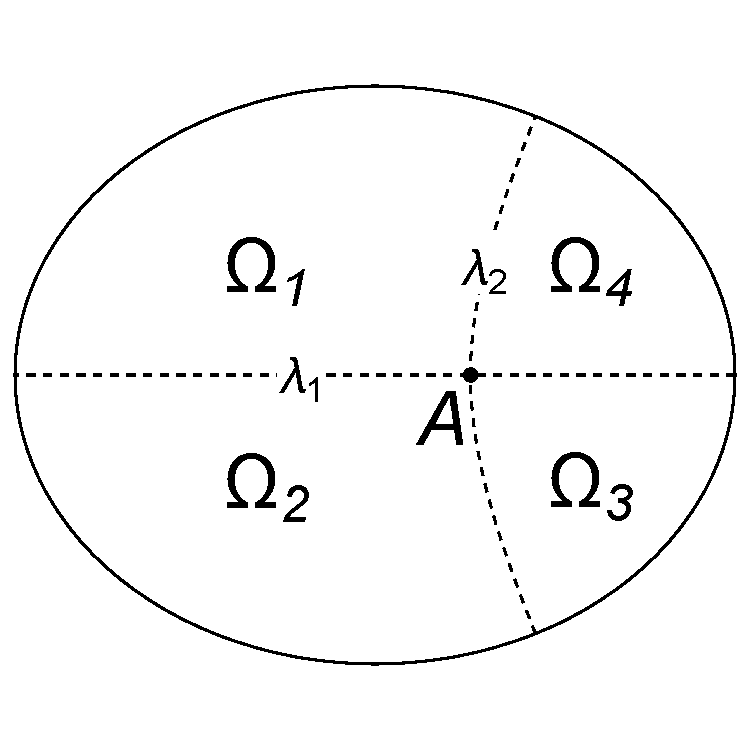
\includegraphics[width=0.35\textwidth]{images/ch4/section1/img2.pdf}
\caption{Взаимное расположение областей $\Omega_1,\ldots,\Omega_4$.}
    \label{fig:pt8:_example6}
\end{figure}

Предположим, что внутренность эллипса разделена на области дугами софокусных квадрик таким образом, что имеются всего одна точка их пересечения, которую обозначим $A$.
Занумеруем области против часовой стрелки $\Omega_1, \ \Omega_2, \ \Omega_3, \ \Omega_4$ (см. рис. \ref{fig:pt8:_example6}).
Пусть общая часть границы $\Omega_1 \cup \Omega_4$ и $\Omega_2 \cup \Omega_3$ --- дуга софокусной квадрики с параметром $\lambda_1$, а общая часть границы $\Omega_1 \cup \Omega_2$ и $\Omega_3 \cup \Omega_4$ --- дуга софокусной квадрики с параметром $\lambda_2$ (см. рис. \ref{fig:pt8:_example6}).

Введем коэффициент $\gamma_A$ в точке $A$, имеющий смысл коэффициента ветвления, по формуле $$\gamma_A = \lambda_1(n_1^2 - n_2^2) + \lambda_2(n_2^2-n_3^2) + \lambda_1(n_3^2-n_4^2) + \lambda_2(n_4^2-n_1^2) = (\lambda_1 - \lambda_2) ( n_1^2 - n_2^2 + n_3^2 - n_4^2).$$

Определим вспомогательную функцию $\widetilde{\Xi}(x, y, v_x, v_y)$ 

\begin{equation*}
\widetilde{\Xi}(x, y, v_x, v_y) = \left[
\begin{array}{ll}
    \Lambda(x, y, v_x, v_y) n_1^2, \qquad  \  \ \qquad   \text{ если } (x,y) \in \Omega_1 
    \\
    \Lambda(x, y, v_x, v_y) n_p^2 + \sum_{j=1}^{p-1} \lambda_j(n_j^2-n_{j+1}^2), \\
     \qquad \qquad \qquad \qquad \qquad \qquad  \text{ если } (x,y) \in \Omega_p \text{ для } 1 < p \leq 4. 
\end{array}
\right.
\end{equation*}
Неформально говоря, она почти подходит на роль дополнительного интеграла, но имеет разрыв на дуге, разделяющей области $\Omega_1$ и $\Omega_4$. Можно проверить, что на любой бильярдной траектории, пересекающей эту дугу, функция $\widetilde{\Xi}$ испытывает один и тот же скачок, равный  $\pm \gamma_A$. 
Поэтому мы определим \textit{первый интеграл $\Xi(x, y, v_x, v_y)$ со значениями в $S^1= \mathbb{R}/\gamma_A \mathbb{Z}$ }по формуле $$\Xi(x, y, v_x, v_y) = \widetilde{\Xi}(x, y, v_x, v_y) \mod \gamma_A.$$
Эта величина на траекториях бильярда сохраняется.
\bigskip

Если границы раздела областей пересекаются по двум и более точкам, то имеет место общая закономерность: 
\medskip

\textit{ 
\noindent Для каждой точки пересечения $A_i, i=1,\ldots,m$, определен коэффициент $\gamma_{A_i}$. Дополнительный интеграл \  $\Xi(x, y, v_x, v_y)$ принимает значения в $\mathbb{R}/(\gamma_{A_1} \mathbb{Z}+ \ldots + \gamma_{A_m} \mathbb{Z})$. Если $\gamma_{A_i}$ соизмеримы, т. е. всевозможные дроби $\dfrac{\gamma_{A_i}}{\gamma_{A_j}}$ --- рациональные числа (или бесконечность), то $\mathbb{R}/(\gamma_{A_1} \mathbb{Z}+ \ldots + \gamma_{A_m} \mathbb{Z}) = S^1$. Если же среди $\gamma_{A_i}$ есть пара с иррациональным отношением $\dfrac{\gamma_{A_i}}{\gamma_{A_j}}$, то подгруппа $\gamma_{A_1} \mathbb{Z}+ \ldots + \gamma_{A_m} \mathbb{Z}$ всюду плотна в $\mathbb{R}$. В этом случае дополнительный интеграл $\Xi(x, y, v_x, v_y)$ корректно определен, но использовать его для топологического анализа структуры траекторий представляется весьма затруднительным.}

\bigskip
\textit{ Случай 2: две точки пересечения.}
\begin{figure}[!htb]
\centering
   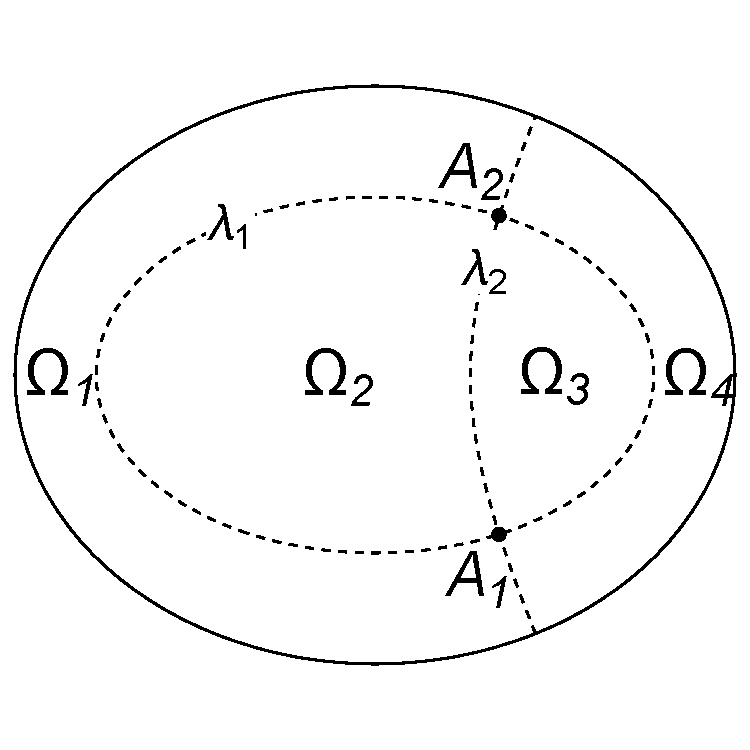
\includegraphics[width=0.35\textwidth]{images/ch4/section1/img3.pdf}   
    \caption{Взаимное расположение областей $\Omega_1, \ldots, \Omega_4$.}
    \label{fig:pt8:_example7}
\end{figure}
Рассмотрим области, изображенные на рис. \ref{fig:pt8:_example7}. 
Легко вычислить коэффициенты $\gamma_{A_1}$ и $\gamma_{A_2}$ в точках $A_1, A_2$ (т.е. скачки дополнительного интеграла при обходе против часовой стрелки вокруг соответствующей точки):
$$\gamma_{A_1} = \lambda_2(n_1^2 - n_4^2) + \lambda_1(n_4^2-n_3^2) + \lambda_2(n_3^2-n_2^2) + \lambda_1(n_2^2-n_4^2), $$
% = (\lambda_2 - \lambda_1) ( n_1^2 - n_2^2 + n_3^2 - n_4^2),$$
$$\gamma_{A_2} = \lambda_1(n_1^2 - n_2^2) + \lambda_2(n_2^2-n_3^2) + \lambda_1(n_3^2-n_4^2) + \lambda_2(n_4^2-n_1^2). $$
% = (\lambda_1 - \lambda_2) ( n_1^2 - n_2^2 + n_3^2 - n_4^2).$$
Как видно, в этом случае $$\gamma_{A_1} = -\gamma_{A_2}.$$
Поэтому дополнительный интеграл $\Xi(x, y, v_x, v_y)$, сохраняющийся на траекториях бильярда, может быть задан по модулю $\gamma_{A_1}$ формулой $\Xi = \widetilde{\Xi} \mod \gamma_{A_1}$, где 
\begin{equation*}
\widetilde{\Xi}(x, y, v_x, v_y) = \left[
\begin{array}{ll}
    \Lambda(x, y, v_x, v_y) n_1^2,  \qquad \ \  \qquad  \text{ если } (x,y) \in \Omega_1 
    \\
    \Lambda(x, y, v_x, v_y) n_p^2 + 
    \sum_{j=1}^{p-1} \lambda_j(n_j^2-n_{j+1}^2), \\
     \qquad \qquad  \qquad \qquad  \qquad \qquad \text{ если } (x,y) \in \Omega_p \text{ для } 1 < p \leq 4. 
\end{array}
\right.
\end{equation*}
 \medskip
\textit{ Случай 3: две точки пересечения.}
Рассмотрим области, изображенные на рис. \ref{fig:pt8:_example8}. 
\begin{figure}[!htb]
\centering
   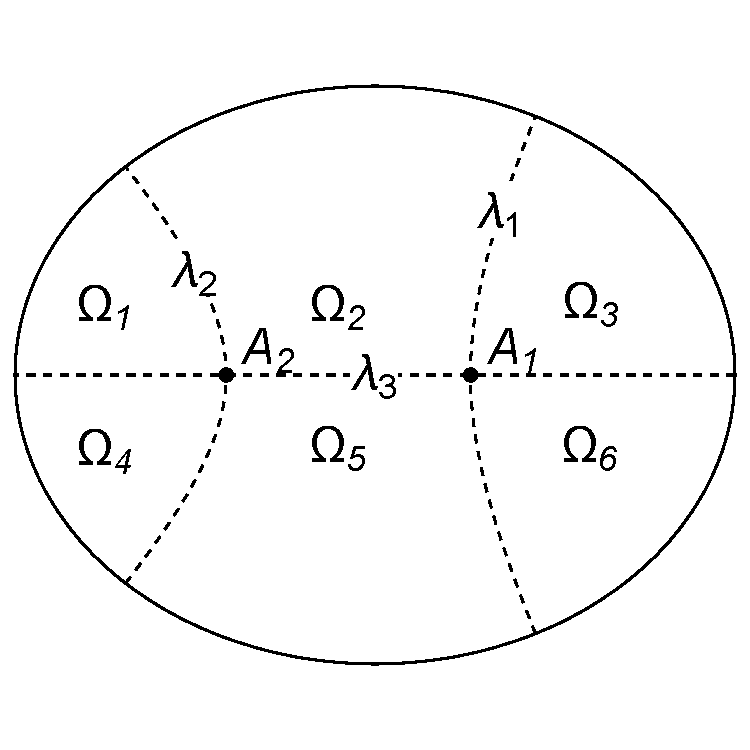
\includegraphics[width=0.35\textwidth]{images/ch4/section1/img4.pdf}   
    \caption{Взаимное расположение областей $\Omega_1, \ldots, \Omega_6$.}
    \label{fig:pt8:_example8}
\end{figure}


Легко видеть, что коэффициенты $\gamma_{A_1}, \gamma_{A_2}$ в точках $A_1$, $A_2$, соответственно, задаются формулами:
$$\gamma_{A_1} = (\lambda_3 - \lambda_1)(n_2^2 - n_5^2 + n_6^2 - n_3^2),$$
$$\gamma_{A_2} = (\lambda_3 - \lambda_2)(n_1^2 - n_4^2 + n_5^2 - n_2^2).$$

В зависимости от значений параметров отношение $\dfrac{\gamma_{A_1}}{\gamma_{A_2}}$ может быть как рациональным, так и иррациональным.

Роль коэффициента $\gamma_A$ проявляется в следующей задаче, которую мы решим в рамках настоящей статьи.

\textbf{Задача Б.} Рассмотрим в качестве бильярдной области $\Omega$  <<прямоугольник>>, образованный дугами концентрических окружностей $BC$, $AD$ и отрезками вертикально проведенного диаметра $AB$ и $CD$. (см. рис. \ref{fig:pt8:_example9}).
Область $\Omega$ разбивается на две части дугой  $EF$ концентрической окружности  и отрезком $FG$ горизонтально проведенного диаметра. Нумерация областей показана на рис. \ref{fig:pt8:_example9}.

Требуется описать как изоэнергетическое многообразие расслаивается на поверхности уровня первого интеграла $\Xi$.


\begin{figure}[!htb]
\centering
   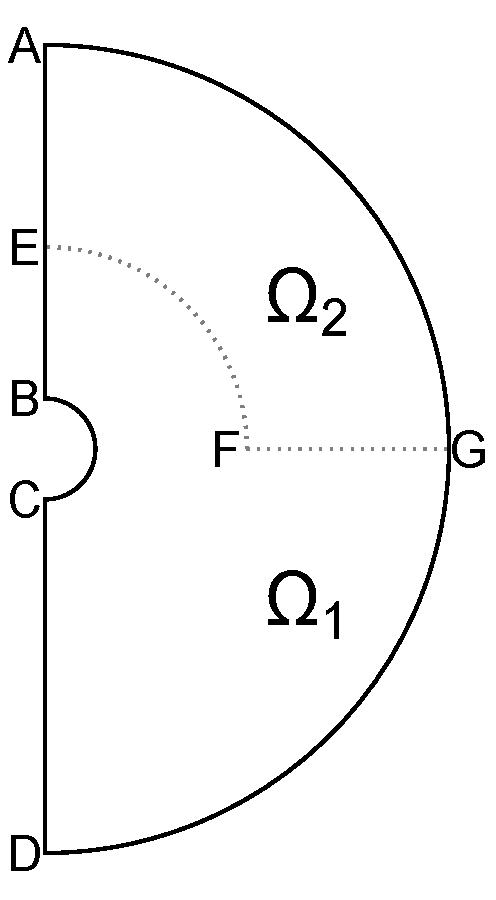
\includegraphics[width=0.25\textwidth]{images/ch4/section1/imgB.pdf}   
    \caption{Взаимное расположение областей $\Omega_1, \Omega_2$.}
    \label{fig:pt8:_example9}
\end{figure}

%Перечислим основные результаты настоящей работы.
%Для задачи А полностью описаны поверхности уровня регулярных значений интеграла $\Xi$ (теорема \ref{st:pt9:n1_n2_surfaces}).
%В разделе \ref{sec:ch4/sec2/subsec2} описаны поверхности уровня для всех нерегулярных значений интеграла $\Xi$, а также все перестройки поверхностей уровня интеграла при проходе через сингулярные значения. 
%Для задачи Б  показано, что многозначный интеграл $\Xi$ в действительности принимает лишь конечное число значений, в теоремах \ref{th:pt10:th1} и \ref{th:pt10:th2} и подразделе \ref{sec:ch4/sec3/subsec8} полностью описаны поверхности уровня регулярных значений интеграла $\Xi$.
%Описанию особых слоев и перестроек посвящен подраздел \ref{sec:ch4/sec3/subsec10}.

\clearpage
